\documentclass[
	% oneside,
	twoside,
	parskip=half,
	% 10pt,
	a4paper,
]{scrbook}

\pdfcompresslevel=0
\pdfobjcompresslevel=0

\usepackage{xcolor}
\definecolor{seeblau}{HTML}{00A9E0}
\definecolor{seegrau}{HTML}{9AA0A7}

\definecolor{seeblau1}{HTML}{CCEEF9}
\definecolor{seeblau2}{HTML}{A6E1F4}
\definecolor{seeblau3}{HTML}{59C7EB}
\definecolor{seeblau4}{HTML}{00A9E0}
\definecolor{seeblau5}{HTML}{008ECE}


\usepackage{graphicx}
\usepackage{amsmath}
\usepackage{subcaption}
\usepackage{wrapfig}
\usepackage[english]{babel}
\usepackage{blindtext}
\usepackage{marginnote}
\usepackage{microtype}
\usepackage{siunitx}
\usepackage[utf8]{inputenc}
\usepackage{csquotes}
\usepackage{nicefrac}
\usepackage[T1]{fontenc}

\usepackage{siunitx}

% select serif font ###########################################################
% \usepackage[rm]{libertinus-type1}
% \usepackage{libertinus}
% \usepackage{roboto-serif}
\usepackage{libertinus}
% \usepackage[sfdefault, scaled=1.05]{biolinum}
% \usepackage{charter}	% designed for 300dpi print
% select sans serif font ######################################################
\usepackage{roboto}
% select math font ###########################################################
% \usepackage{newtxmath}
% \usepackage{sfmath} % sans serif math based on fira sans?
% \usepackage{eulervm}
% \usepackage[scaled=1.063]{libertinust1math}
% \usepackage{notomath}
% \usepackage{unicode-math}
\usepackage{amsfonts}
\usepackage{amssymb}
\usepackage{todonotes}


\setkomafont{disposition}{\normalfont\sffamily}

% not recommended with KOMA-script
\usepackage{tocloft}
\renewcommand\cftchappagefont{\normalfont}
\renewcommand\cftchapfont{\normalfont}
\renewcommand\cftchappresnum{\bfseries}
\renewcommand\cftchapaftersnum{}
\renewcommand{\cftchapfont}{\sffamily}
\renewcommand{\cftsecfont}{\sffamily}
\renewcommand{\cftsubsecfont}{\sffamily}
\renewcommand{\cftchappagefont}{\sffamily}
\renewcommand{\cftsecpagefont}{\sffamily}
\renewcommand{\cftsubsecpagefont}{\sffamily}

% caption
\usepackage{caption}
\captionsetup{
	% font={sf},
	labelfont={sf, bf, color=seeblau},
	labelsep=quad,
	labelformat=simple,
}

% links
\usepackage{hyperref}
\hypersetup{
	colorlinks=true,
	linkcolor=seeblau,
	citecolor=seeblau,
	urlcolor=seeblau,
	% hidelinks=true
}

% bibliography
\usepackage[
	style=numeric-comp, % comp = compressed 4,5,6,7 -> 4-7
	sorting=none,		% Sort by appearance
	% autocite = superscript,
	% backref=true,
	hyperref=true,
	url=true,
	maxbibnames=100
]{biblatex}
\addbibresource{../literature.bib}
\DefineBibliographyStrings{english}{%
    backrefpage  = {see p.}, % for single page number
    backrefpages = {see pp.} % for multiple page numbers
}

% remove issue
\AtEveryBibitem{%
  \clearfield{number}
}

\usepackage{float}
% \floatplacement{figure}{h}
% \floatplacement{table}{H}

% loosen float placement rules
\renewcommand{\topfraction}{0.8}
\renewcommand{\bottomfraction}{.8}
% \renewcommand{\textfraction}{0.1}
\renewcommand{\floatpagefraction}{.9}
% make floats less likely to be placed on a separate page
% \setcounter{totalnumber}{9}
% \setcounter{topnumber}{9}
% \setcounter{bottomnumber}{9}

% decrease space between floats and text
% \setlength{\textfloatsep}{0.5cm}
% \setlength{\floatsep}{0.5cm}
% % decrease space between figure and caption
% \setlength{\abovecaptionskip}{0.2cm}
% \setlength{\belowcaptionskip}{0.2cm}


\usepackage{adjustbox}

\usepackage{datetime}
\newdateformat{dotdate}{
	\twodigit{\THEDAY}.\twodigit{\THEMONTH}.\THEYEAR
}
\newdateformat{monthyeardate}{%
  \monthname[\THEMONTH] \THEYEAR}

% header and footer

\usepackage[
  markcase=noupper
]{scrlayer-scrpage}% activates pagestyle scrheadings automatically
\clearpairofpagestyles
\setkomafont{pageheadfoot}{\normalfont\sffamily}
\setkomafont{pagenumber}{\normalfont\sffamily}
\chead*{\color{seegrau} Draft \dotdate\today}
\ofoot*{\pagemark}
\ohead*{\rightmark}


\title{Optical signature of magnetic phase transition in transition metal phosphorus sulfides}
\subtitle{Bachelor Thesis}
\author{Leon Oleschko}

\begin{document}
\frontmatter
\begin{titlepage}
	% add university logos
	\begin{minipage}{.49\textwidth}
		\raggedright
		% \includegraphics[height=20mm]{../figures/logo/UniWarsaw.png}
		\hspace{2cm}
	\end{minipage}
	\begin{minipage}{.49\textwidth}
		\raggedleft
		% \includegraphics[height=20mm]{../figures/logo/UniKonstanz_Logo.pdf}
	\end{minipage}

	\raggedright
	\sffamily

	\vspace{2cm}
	\newcommand{\markieren}[4]{
		\adjustbox{padding=3pt, bgcolor=seeblau1, margin=-1pt}{\strut{\sffamily\robotoMedium{#1}}}\\
		\adjustbox{padding=3pt, bgcolor=seeblau2, margin=-1pt}{\strut{\sffamily\robotoMedium{#2}}}\\
		\adjustbox{padding=3pt, bgcolor=seeblau3, margin=-1pt}{\strut{\sffamily\robotoMedium{#3}}}\\
		\adjustbox{padding=3pt, bgcolor=seeblau4, margin=-1pt}{\strut{\sffamily\robotoMedium{#4}}}
	}
	{
		\fontsize{32}{32}
		\markieren{Optical signatures of}{magnetic phase transitions}{in transition metal}{phosphorus sulfides}
	}

	\vspace{.25cm}
	{
		\Large
		Bachelor Thesis of Leon Oleschko\\
		% \normalsize\vspace{.25cm}
		Submitted to the Faculty of Physics, Universität Konstanz\\
		May, 2024
	}

	% \vspace{.5cm}
	% \centering
	% \includegraphics[height=20mm]{../figures/logo/UniKonstanz_Logo.pdf}

	\vfill
	\normalsize
	\raggedleft
	% \monthyeardate\today, 
	supervised by Dr. Mateusz Goryca, University of Warsaw\\
	evaluated by Prof. Dr. Sebastian Gönnenwein, Universität Konstanz

\end{titlepage}

\cleardoublepage
\section*{Summary}
Antiferromagnetic van der Waals layered semiconductors such as transition metal phosphorus sulfides are of great interest due to their unique combination of magnetic, optical, and structural properties. 
The layered structure allows for exfoliation and the study of property changes over the transition from three-dimensional to two-dimensional structures.
The exotic thickness-dependent magnetic orders \cite{AFM_review} are influenced by the varying magnetic and structural anisotropies for different materials \cite{MPS_magnetism, CrPS4_magnetic}.
As the selected semiconductors have bandgaps in the optical and near-infrared, optical measurement techniques offer opportunities for fast in situ measurements of the magnetic structure on a limited sample volume.\\
In this work, polarization-resolved photoluminescence spectroscopy has been identified as the most promising optical measurement technique for studying the magnetic phase transitions in the selected materials.
The magnetic splitting of the photoluminescence line of NiPS$_3$ has been demonstrated to be more complex than previously reported, with varying splitting, dependent on the linear polarization.
In CrPS$_4$ the circular dichroism of the photoluminescence line was shown to be proportional to the magnetization, which allows the entire magnetic phase diagram to be studied with optical methods.

\vfill
\section*{Zusammenfassung}
Antiferromagnetische van-der-Waals Halbleiter wie Übergangsmetallphosphorsulfide sind aufgrund ihrer einzigartigen Kombination von magnetischen, optischen und strukturellen Eigenschaften von großem Interesse. 
Deren Schichtstruktur ermöglicht die Exfoliation und die Untersuchung von Eigenschaftsänderungen beim Übergang von dreidimensionalen zu zweidimensionalen Strukturen.
Die exotischen dickenabhängigen magnetischen Ordnungen \cite{AFM_review} werden durch die unterschiedlichen magnetischen und strukturellen Anisotropien für verschiedene Materialien beeinflusst \cite{MPS_magnetism, CrPS4_magnetic}.
Da die ausgewählten Halbleiter, Bandlücken im optischen und nahen infrarot Bereich aufweisen, bieten optische Messtechniken die Möglichkeit, die magnetische Struktur in einem begrenzten Probenvolumen schnell in situ zu messen.\\
In dieser Arbeit wurde die polarisationsaufgelöste Photolumineszenzspektroskopie als die vielversprechendste optische Messtechnik zur Untersuchung der magnetischen Phasenübergänge in den ausgewählten Materialien identifiziert.
Die magnetische Aufspaltung der Photolumineszenzlinie von NiPS$_3$ hat sich als komplexer erwiesen als bisher berichtet, mit einer variierenden Aufspaltung in Abhängigkeit von der linearen Polarisation.
Bei CrPS$_4$ wurde gezeigt, dass der Zirkulardichroismus der Photolumineszenzlinie proportional zur Magnetisierung ist, wodurch das gesamte magnetische Phasendiagramm mit optischen Methoden untersucht werden kann.
\vfill

\clearpage
\section*{Acknowledgements}
This thesis is part of the Bachelor's program in physics at the Universität Konstanz.

I am grateful for the welcoming atmosphere and the opportunity to delve into university research provided by Prof. Dr. Sebastian Gönnenwein's group at the Universität Konstanz prior to this project.
This gave me the opportunity to work on my thesis at the University of Warsaw for three and half months under the supervision of Dr. Mateusz Goryca.
I would like to thank Prof. Dr. Sebastian Gönnenwein and Dr. Mateusz Goryca for making this experience possible.\\
I am especially grateful to Dr. Mateusz Goryca, who despite his busy schedule was always willing to help me.
His mentorship and encouragement, along with the freedom to explore independently, have been invaluable.\\
I would also like to thank the members of the group for their support and the opportunity to learn from them.
In particular, Jan Suffczyński for helping me with the transmission measurements, Tomasz Kazimierczuk who helped with all sorts of technical issues, and Julia Kucharek for helping me with the atomic force microscope.

\cleardoublepage
{
	\sffamily
	\hypersetup{hidelinks}
	\tableofcontents
}

\mainmatter

\chapter{Introduction}
\begin{wrapfigure}[21]{O}{.4\textwidth}
	\includegraphics[width=.4\textwidth]{../../figures/crystal structures/NiPS3 3d.png}\\
	\caption{}
	Crystal structure of NiPS$_3$ as an example for the studied materials.
	Weakly bonded layers in the $a$-$b$ plane are held together by van der Waals forces along the $c$ axis.
	The image is adapted from \cite{NiPS3_coherent}.
	\label{fig:crystal structure}
\end{wrapfigure}

Antiferromagnetic van der Waals materials such as transition metal phosphorus sulfides are of great interest due to their unique combination of magnetic, optical, and structural properties \cite{MPX_review}. 
The structure of a specific material, NiPS$_3$, is illustrated in \autoref{fig:crystal structure} \cite{NiPS3_coherent}, demonstrating strong layers in the $a$-$b$ plane, bonded by weak van der Waals interactions along the $c$ axis.
This allows for mechanical exfoliation of the flakes and enables the investigation of property changes over the transition from three-dimensional to two-dimensional structures \cite{MPX_review}.
The magnetic properties of these materials are dominated by the spin direction of the transition metal ions in the lattice \cite{MPS_magnetism}.
They exhibit a wide range of thickness-dependent exotic magnetic orders \cite{AFM_review}, influenced by the varying anisotropy for different materials \cite{MPS_magnetism, CrPS4_magnetic}.\\
However, determining these orders is challenging due to the antiferromagnetic structure, which results in a net magnetization of zero \cite{MPX_review,MPS_magnetism,afm}.
Especially fast measurements in the monolayer limit without disturbing the sample is difficult \cite{AFM_review, CrPS4_magnetic}, but important for studying phase changes and exploring applications in spintronics \cite{AFM_review}.
Optical measurements emerge as the most promising methods, as they can be used in situ, on a small sample volume, and offer spatial resolution. 
However, the commonly used Kerr effect faces limitations, as detecting small polarization rotations in thin layers, in the order of \SI{5}{\mu rad} has a low signal-to-noise ratio \cite{AFM_review}. \todo{better wording?}\\
The goal of this project is to identify optical signatures of magnetic order or magnetic phase transitions in selected transition metal phosphorus sulfides, with the aim of developing a method suitable for fast in situ measurements of the magnetic structure in monolayers in the future.
This project focuses on identifying and demonstrating a promising measurement technique, rather than on studying the magneto-dependent light-matter interaction process.

Various optical measurement techniques were evaluated in the methodology section, with polarization-resolved photoluminescence spectroscopy identified as the most promising method.
Subsequently, this method was applied to NiPS$_3$ and CrPS$_4$ in the results section.\\
While the phase transition in NiPS$_3$ was out of the experimental capabilities, the circular dichroism of the photoluminescence in CrPS$_4$ was used to observe phase transitions.
The results also demonstrate the limits of our current theoretical understanding of the photoluminescence process in these materials. 

% paragraph that first some background about the used materials is given
\section{Properties of the selected materials}
\todo[inline]{}
% An introduction to the materials utilized in this project is given with a brief explanation of their magnetic and optical properties.
The selected materials belong to the class of transition metal phosphorus sulfides or transition metal thiophosphates \cite{MPS_magnetism}, which are a subset of the broader category of transition metal chalcogenides (TMD).
TMDs share a similar crystal structure but differ in the chalcogenides they contain. 
They also exhibit different magnetic orders than antiferromagnetic \cite{AFM_review}.
The materials chosen for this project are NiPS$_3$, CrPS$_4$, MnPS$_3$, and FePS$_3$.
They were selected for their wide range of magnetic anisotropies \cite{MPS_magnetism,CrPS4_magnetic}.

% \subsection{Magnetic Properties}
% define antiferromagnetic order
The magnetic properties of transition metal phosphorus sulfides are dominated by the spins of the transition metal ions in the lattice \cite{MPS_magnetism}.
In the absence of an external magnetic field $B$ and below the Néel temperature $T_N$, the magnetic order of the spins is antiferromagnetic.
In this phase, the spins of the ions align in two or more sublattices, resulting in a net magnetization of zero \cite[p.195]{afm}. 
This order can be altered by applying a sufficiently strong external magnetic field $H$ to induce a magnetic phase transition, in which the spins align with the field \cite{CrPS4_magnetic}.
Alternatively, the magnetic order can be altered by changing the temperature, as the Néel temperature is the temperature at which the magnetic order changes from antiferromagnetic to paramagnetic \cite{MPS_magnetism, CrPS4_magnetic}.

% \subsection{Optic Properties}
% define bandgap, mention that it splits in magnetic field \cite{MPX_first_principles}
All studied materials are semiconductors with a bandgap $E_B$ in the visible to near-infrared range.
The bandgap is the energy difference between the valence and conduction bands, which determines the energy required to excite an electron from the valence to the conduction band.
For a photon to be absorbed by the semiconductor, the photon energy $E_\text{ex} = h\nu = \nicefrac{hc}{\lambda}$ must exceed the bandgap $E_B$.
A change in the order of \SI{1}{meV} of the band edges in response to the alignment of the spins of the metal ions is expected according to theoretical calculations \cite{MPX_first_principles}.
Therefore, the bandgap is expected to change in response to the magnetic order.
% explain photoluminescence as a direct 

% with exciton 




% Wannier–Mott exciton
% explain possible splitting and polarization with Zeeman effect of exciton 
% mention that there are other models for the photoluminescence process



% \clearpage

% Two-dimensional materials feature unique properties, which makes them attractive for applications in nanocatalysis, optoelectronics, and spintronics \cite{MPX_review}.
% The class of \textit{transition metal phosphorus sulfides} offers a combination of properties that make them an ideal subject for the study of two-dimensional materials.
% These materials exhibit a wide range of exotic magnetic orders \cite{AFM_review}.

% MPS$_x$ "lowest electronic transition is mostly of d-d character and is localized at the transition-metal atoms." \cite{CrPS4_pl}.

% The crystal structure of one of the studied materials, NiPS$_3$, is illustrated in \autoref{fig:crystal structure} taken from \cite{NiPS3_coherent}.
% This structure is referred to as a \textit{van der Waals} layered material, as the material is highly anisotropic with quasi-2D layers held together by weak van der Waals forces.
% The layers are easy to mechanically exfoliate, which allows the manufacture of samples with a thickness down to monolayers \cite{NiPS3_few_layer}.\\
% The materials NiPS$_3$, CrPS$_4$, MnPS$_3$, and FePS$_3$ were chosen,  
% as these materials exhibit a wide range of different magnetic behaviors because the anisotropy of the magnetic interaction is different in each material \cite{MPS_magnetism,CrPS4_magnetic}.
% The magnetic properties are dominated by the spins of the metal ions in the lattice \cite{MPS_magnetism, NiPS3_magnon_gap, CrPS4_magnetic}.\\
% In NiPS$_3$ the interlayer coupling is weak and the spins of the Ni$^{2+}$ ions are in the layer planes \cite{MPS_magnetism}.
% In contrast, CrPS$_4$ exhibits strong interlayer coupling and has a magnetic structure that is perpendicular to the layers \cite{CrPS4_magnetic}.
% The combination of this property together with easy exfoliation is promising, as it allows to alter the magnetic properties of the material.

% The magnetic structure of all studied materials at low external magnetic field and below the Néel temperature of \SI{155}{K} for NiPS$_3$ and \SI{38}{K} for CrPS$_4$ \cite{MPS_magnetism, CrPS4_magnetic}  is anti-ferromagnetic.\\
% In the anti-ferromagnetic phase, two sublattices align in opposite directions, resulting in a magnetization of $M=0$.\\
% Over the Néel temperature, the magnetic order is paramagnetic with the spins randomly oriented and $M=0$.\\
% When a sufficiently strong external magnetic field $H>H_\text{SF}$ is applied a \textit{magnetic phase transition} occurs, known as a spin-flop transition.
% In this transition, all spins align with the magnetic field, resulting in a phase change from antiferromagnetic to ferromagnetic with $\vec{H}\propto \vec{M}>0$.\\
% This happens for CrPS$_4$ at \SI{7.5}{T} \cite{CrPS4_magnetic} and for NiPS$_3$ at \SI{14}{T} \cite{NiPS3_magnon_gap}.
% Unfortunately, the experimental capabilities were limited to \SI{10}{T}.

% The selected materials offer useful optical properties, as they are semiconductors with a bandgap $E_B$ in the visible to near-infrared range.
% Consequently, they are suitable for optical measurements.\\
% Which have the advantage, that they can be used for fast, in situ measurements on a small sample volume or even with spatial resolution.\\
% This allows the study of changes in the fast anti-ferromagnets through pump-probe or noise measurements \cite{AFM_review}.

% The temporal resolution is constrained by the speed of the material-light interaction.\\
% For an excitation photon to be absorbed by a semiconductor the photon energy $E_\text{ex} =h\nu= \nicefrac{hc}{\lambda}$ must exceed that of the bandgap $E_B$.
% This results in the excitation of an electron $e^-$ from the valence band to the conduction band, accompanied by the creation of a hole $h^+$ in the valence band.\\
% The electron and the hole can combine to form a neutral exciton $x$, a bound state of the electron and the hole, with a binding energy $E_x$.\\
% Additionally, more complex structures such as charged excitons or biexcitons, can form with different binding energies.
% All these structures can also be in excited states.\\
% The energy difference $E_\text{ex}-E_B+E_x$ is dissipated through processes such as phonon emission, which heats the sample, intra-band photon emission, or a combination of these mechanisms.\\
% The remaining energy is emitted as a luminescence photon with energy $E_B - E_x$, which can be observed as one strong peak in the spectrum for excitons and multiple smaller ones for the more complex structures.
% \cite{MPX_first_principles,NiPS3_anisotropic,NiPS3_coherent,NiPS3_exciton}

% When a local magnetic field $B=H+M$ is present, the luminescence line splits into two lines with different energies.
% This phenomenon can be explained by the Zeeman effect or spin-orbit coupling of the exciton \cite{NiPS3_exciton}.\\
% In addition, the bandgap also changes in response to the magnetic field \cite{MPS_magnetism}. 
% This change can vary depending on the spin directions.
% Therefore, changes for different circular polarizations can be expected \cite{MPX_first_principles}.\\
% Various models have been proposed to explain the linear polarisation of the luminescence \cite{NiPS3_coherent, NiPS3_linear, NiPS3_exciton, NiPS3_anisotropic}.

% The objective of this project is to identify optical signatures of the magnetic phase transition in the selected materials using a measurement technique that can be used for fast in situ measurements and on monolayers in the future.\\
% This will enable further studies of the magnetic properties with temporal resolution through pump-probe or noise measurements, which is particularly relevant for spintronics applications \cite{AFM_review}.



\chapter{Methodology}
\section{Sample Preparation}
The samples of all studied materials were prepared as a first step of the presented work.
Initially, measurements were conducted on polycrystalline bulk crystals.
However, to create a cleaner surface and increase the probability of obtaining monocrystalline flakes, the crystals were later exfoliated.

\begin{figure}
	\centering
	\begin{subfigure}[t]{.24\textwidth}
		\vskip 0pt
		\includegraphics[width=\textwidth]{../../photos/bulk_sample.jpg}
		\caption{Small bulk crystals in \SI{2}{cm} vials.}
		\label{fig:samples_vials}
	\end{subfigure}
	\begin{subfigure}[t]{.24\textwidth}
		\vskip 0pt
		\includegraphics[width=\textwidth]{../figures/mounted_bulk_samples.jpg}
		\caption{Strain-free mounted bulk crystals. The crystals are under the black paper.}
		\label{fig:samples_bulk_mounted}
	\end{subfigure}
	\begin{subfigure}[t]{.24\textwidth}
		\vskip 0pt
		\includegraphics[width=\textwidth]{../../data/2023-11-02/i005_NiPS3_50x-scalebar.png}
		\caption{Typical smooth surface with characteristic features from the hexagonal crystal lattice (NiPS$_3$). Scalebar \SI{10}{\mu m}}
		\label{fig:bulk_nips3}
	\end{subfigure}
	\begin{subfigure}[t]{.24\textwidth}
		\vskip 0pt
		\includegraphics[width=\textwidth]{../../data/2023-11-02/i009_FePS3_100x-scalebar.png}
		\caption{Unexpected rough surface of FePS$_3$, probably due to contamination.  Scalebar \SI{10}{\mu m}}
		\label{fig:bulk_feps3}
	\end{subfigure}
	\caption{Photos of the bulk samples.}
\end{figure}

% The growing of the bulk crystals using the vapor transport method, a conventional manufacturing technique for these materials \cite{MPX_review, AFM_review}, is not part of this work.
Prior to this work, bulk crystals of various transition metal phosphorus sulfides were grown using the vapor transport method, a conventional manufacturing technique for these materials \cite{MPX_review, AFM_review}.\\
They are shown as they were at the beginning of this work in \autoref{fig:samples_vials}, with approximate dimensions of $4 \times 2 \times \SI{.5}{mm}$.
The thickness was quantified using thin-film interference, as detailed in Section \ref{sec:thickness}.\\
For the first measurements, the samples were mounted strain-free on a copper holder.
They were fixed with a piece of black paper with a hole, that was glued to the copper holder at the corners, as shown in Figure \autoref{fig:samples_bulk_mounted}.
Upon examination under a microscope, the surface of the NiPS$_3$, CrPS$_4$, and MnPS$_3$ samples appeared smooth, as shown in \autoref{fig:bulk_nips3}, while the FePS$_3$ sample exhibited a rough surface as depicted in \autoref{fig:bulk_feps3}.
The roughness appeared to result from contamination by an oxidized layer, as it could be removed by mechanical exfoliation.


\subsection{Exfoliation}
\begin{figure}
	\centering
	\begin{subfigure}[t]{.3\textwidth}
		\vskip 0pt
		\includegraphics[width=\textwidth]{../../photos/exfoliation.jpg}
		\caption{First Step: subdividing the bulk crystal multiple times.}
		\label{fig:exfoliation_division}
	\end{subfigure}
	\begin{subfigure}[t]{.3\textwidth}
		\vskip 0pt
		\includegraphics[width=\textwidth]{../../photos/exfoliation glass.jpg}
		\caption{Second Step: transferring the flakes to a substrate.}
		\label{fig:exfoliation_transfer}
	\end{subfigure}
	\begin{subfigure}[t]{.3\textwidth}
		\vskip 0pt
		\includegraphics[width=\textwidth]{../../data/2023-12-04_LO_MG_NiPS3/CrPS4_50x_10um.png}\\
		\caption{Result: CrPS$_\text{4}$ flakes on Si/SiO$_\text{2}$ substrate, Scalebar 10$\mu$m}
		\label{fig:exfoliation_result}
	\end{subfigure}
	\caption{Photos at different stages in the exfoliation process.}
	\label{fig:exfoliation}
\end{figure}
To achieve a cleaner surface, especially crucial for the FePS$_3$ crystals, and to increase the likelihood of obtaining monocrystalline flakes, the bulk crystals were mechanically exfoliated.
The stages of this process are photographed in \autoref{fig:exfoliation}.

Initially, an as-grown bulk crystal with thickness $d_0$ is placed on adhesive tape.
Subsequently, a second piece of tape is placed on top of the crystal and removed, causing the crystal to split into two flakes that adhere to the two pieces of tape.
The flakes already on the tape are divided each time this is repeated into thinner flakes with the average thickness $\left< d_{n} \right> = \nicefrac{1}{2} \left< d_{n-1} \right>$.
For most samples, the number of repetitions $n$ was $8$.
This step is depicted in \autoref{fig:exfoliation_division}.
The technique allows to produce monolayers with $ \left<d_n\right>  = \SI{0.8}{nm}$ \cite{NiPS3_few_layer} from a $d_0 = \SI{400}{um}$ thick crystals, requiring just $n = \log_2 \nicefrac{d_0}{\left<d_n\right>} \approx 19$ steps.\\
Finally, the flakes are transferred to a substrate.
In \autoref{fig:exfoliation_transfer} the flakes are transferred to a glass substrate.
In this step, only the thinner flakes adhere to the substrate when the tape is removed, as they are more flexible and can better deform to the substrate.
The ratio of adhesion between the flakes and the substrate and the flakes and the tape determines the yield of flakes that remain on the substrate.
The utilized adhesive tape, \textit{Nitto Denko ELP BT-150E-CM}, was selected for its lowe adhesion.
The adhesion between the flake and the substrate can be tuned by selecting different substrates.
For instance, the yield on glass was $10$ to $100$ times lower than on a Si/Si$_2$ substrate.
To get even more granularity the transfer was tried at elevated temperatures to reduce the adhesion.
To increase the yield even more this transfer step was repeated multiple times for the glass substrate.\\
The results are flakes on a substrate, as seen under a microscope in \autoref{fig:exfoliation_result}.

The resulting flakes exhibit a thickness of approximately $\SI{500}{nm}$, as measured with atomic force microscopy in Section \ref{sec:aligning flakes} (\autoref{fig:AFM}).
When compared to monolayers, these flakes can be considered bulk material.


\section{Measurement Techniques}
To identify a suitable method for investigating the optical properties, various optical spectroscopy techniques were evaluated without applying a magnetic field. \\
As the expected change in the bandgap due to magnetic field is in the order of \SI{1}{meV} according to theoretical calculations \cite{MPX_first_principles}, the techniques should be sensitive to small energy changes.

% \begin{wrapfigure}[18]{O}{.4\textwidth}
% 	\includegraphics[width=.4\textwidth]{../figures/carray schematic.png}\\
% 	\caption\\
% 	Schematic of the transmission spectrometer from \cite{cary}.
% 	\label{fig:carry}
% \end{wrapfigure}
\subsection{Transmission Spectroscopy}
\begin{figure}
	\centering
	\includegraphics{../figures/2024-03-15 MnPS3 transmission raw.pdf}
	\caption{Unprocessed relative transmission spectra for NiPS$_3$ and a calibration Hole. Non-constant relative transmission of the hole with a jump at \SI{1.55}{eV}.}
	\label{fig:transmission raw}
\end{figure}
To begin the exploration of optical spectroscopy techniques, transmission spectroscopy was selected due to its independence from surface quality.
Specifically, a commercial double-beam spectrophotometer, the \textit{Cary 5000}, was employed.
This spectrometer has two user-accessible beam paths, one for reference and the other for the sample.
The spectrometer uses a single light source and two detectors to calculate the relative transmissivity as $T = \nicefrac{I_\text{Sample}}{I_\text{Reference}}$ between the two paths.\\
For the initial measurements, MnPS$_3$ was selected because the \SI{.5}{mm} bulk crystals are already visually transparent.
The relative transmissivity is shown in \autoref{fig:transmission raw} for a MnPS$_3$ crystal and a hole in the sample path. For both measurements the reference path was empty.\\
Surprisingly the relative transmission of the hole is not constant.
The only difference between the paths are the Quartz windows of the cryostat in which the sample was mounted and the aperture of the sample holder.
The non-uniform transmission spectrum observed can be attributed to a wrong calibration of the spectrometer around the transition from infrared to visible mode, occurring at \SI{800}{nm} (corresponding to \SI{1.55}{eV}).\\
Irrespective of the underlying cause, the measurement was reproducible and the signal can be corrected by dividing it with a calibration spectrum of the hole and aligning the visible and infrared spectra in software.
\begin{figure}
	\centering
	\includegraphics{../figures/2024-03-15 MnPS3 transmission processed.pdf }
	\caption{Absorption spectrum ($\approx 1- T$) of MnPS$_3$ corrected with a calibration spectrum. The bandgap can be seen at \SI{2.6}{eV}.}
	\label{fig:transmission corrected}
\end{figure}
The corrected absorption spectrum ($\approx 1 - T$) is depicted in \autoref{fig:transmission corrected} and reproduces the shape of the absorption spectrum in \cite{MnPS3_transmission}.
The bandgap is at \SI{2.6}{eV} above which the spectrometer saturates due to insufficient signal through the sample.

\begin{figure}
	\centering
	\begin{subfigure}[c]{3.5in}
		\vskip 0pt
		\includegraphics{../figures/2024-03-15 Absorbance.pdf}
		\caption{Corrected absorption spectra of different materials. Corresponding with features fond in literature \cite{CrPS4_transmission, NiPS3_transmission, FePS3_transmission}.}
		\label{fig:transmission}
	\end{subfigure}
	\begin{subfigure}[c]{1.5in}
		\vskip 0pt
		\includegraphics[width=\textwidth]{../../photos/transmission samples.jpg}
	\caption{Thick exfoliated samples, with specific transparency to not saturate the spectrometer, mounted with the tape used for exfoliation. From left to right: MnPS$_3$, FePS$_3$, NiPS$_3$, CrPS$_4$}
	\label{fig:transmission samples}
	\end{subfigure}
	\caption{Transmission measurements of multiple samples.}
\end{figure}
For the other samples the features depicted in \autoref{fig:transmission} correspond with those recorded in the literature \cite{CrPS4_transmission, NiPS3_transmission, FePS3_transmission}.
The main problem with this setup is that the spectrometer saturates quickly in the sample or the reference path when the sample is too thin or too thick.
It also has no way to individually display the intensity for the sample or reference path which makes adjustments difficult.
In order to obtain any usable measurements, the samples were exfoliated to a specific optical transparency, as shown in \autoref{fig:transmission samples}.
Additionally, a compensating aperture was placed in the reference beam.
To hold the thick exfoliated flakes, they were not transferred to a substrate but mounted with the adhesive tape used for exfoliation. 
This method was successfully used down to \SI{10}{K} without any issues.
However, this workflow is rather tedious and there is no way to use a magnet with the spectrometer away.\\
There were plans to rebuild the transmission setup using a cryostat with a built-in super-conducting magnet within the presented project, but this was not realized due to time constraints and unexpected measurements discussed in Section \ref{sec:aligning flakes}.
Nevertheless, this technique remains promising as it allows for the independent measurement of the bandgap, circumventing luminescent phenomena.

\clearpage
\subsection{Reflection Spectroscopy}
\begin{figure}
	\centering
	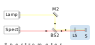
\includegraphics{../figures/setup_reflection.pdf}
	\caption{Setup used for reflection spectroscopy. The light from a halogen lamp is focused by L$_5$ on the sample S in the cryostat and the reflected light is collected through the beam-splitter BS$_2$ by a Spectrometer.}
	\label{fig:reflection setup}
\end{figure}
Subsequently, reflection spectroscopy using the setup shown in \autoref{fig:reflection setup} was evaluated.
In this instance, a halogen lamp was utilized to illuminate the sample.
The light was focused by a lens (L$_5$) with a high numeric aperture on a small (in the order of \SI{10}{um}) spot.
The reflected beam passed through a beam-splitter (BS$_2$) into a spectrometer.
This technique only needs access to the sample from a single side, which simplifies the setup.
\begin{figure}
	\centering
	\includegraphics{../figures/2024-03-14 reflection spectra.pdf}
	\caption{Reflection spectra of bulk crystals with broad spectrum from a halogen lamp used for illumination. Thin-film interference below the bandgap deduced from transmission measurements, shown as vertical lines.}
	\label{fig:reflection spectra}
\end{figure}

The unprocessed recorded spectra for bulk crystals of highly transparent MnPS$_3$ and the material with the most clearly visible bandgap edge (NiPS$_3$), are represented in \autoref{fig:reflection spectra}.
Below the bandgap, the crystals are transparent, and a thin-film interference pattern is visible.\\
Deconvolving the spectral shape of the lamp by dividing the signal from the sample with the spectrum of a mirror was attempted, but the objective lens L$_5$ in \autoref{fig:reflection setup} has a strong chromatic aberration, which alters the spectrum too much.
\begin{figure}
	\centering
	\includegraphics{../figures/2024-03-14 reflection spectra IMF.pdf}
	\caption{Reflection spectra filtered with empirical mode decomposition to eliminate the influence of the light source.}
	\label{fig:reflection filtered}
\end{figure}
In order to remove the lamp spectrum, a filter function $f$, for example, the \textit{Empirical Mode Decomposition}, can be employed \cite{thickness}.
The result of the filtered signal is presented in \autoref{fig:reflection filtered}.
However, even with the filtering, the bandgap edge remains difficult to detect precisely, which makes the technique unsuitable for the detection of the expected small shifts in the bandgap.

\subsubsection{Thickness Estimation}
\label{sec:thickness}
The thin film interference pattern can be utilized to estimate the thickness of the sample.
In order for the total reflection to be strong, the top reflection and the bottom reflection have to be in phase.
Specifically $\nicefrac{2nd}{\lambda}=j$ with the whole cycle offsets $j\in\mathbb{N}$, the refractive index $n$ and $2$ times the thickness $d$.
Therefore the filtered reflected signal is similar to:
\begin{align}
	R(\lambda > \lambda_\text{Bandgap}) &\approx \cos \left( 2 \pi \cdot \frac{2 n d}{\lambda} \right)
\end{align}
which can be decomposed into the components for different thicknesses:
\begin{align}
	S(nd) &= \mathcal{F}\left[ f\left(R\left(\frac{1}{\lambda}\right)\right)\right]( 2 nd)
\end{align}
Where $f$ is the filter function used to remove the influence of the light source.
And the Fourier Transform $\mathcal{F}$ is evaluated using the Lomb-Scargle method \cite{scargle} because the data is not evenly spaced. 
Even for evenly spaced data this method is useful as it is less sensitive to intensity noise than the discrete Fourier transform \cite{scargle}.\\
The NiPS$_3$ samples each have one effective thickness, in the order of \SI{400}{um}.
In contrast, the MnPS$_3$ sample displays multiple peaks in the range of \SI{40}{um}.
When observed with an optical microscope in \autoref{fig:thickness MnPS3}, the MnPS$_3$ sample has multiple layers of cracks at different depths, indicated by the varying focus.
This matches with the recorded thickness signal.
The thickness signal for different samples is depicted in \autoref{fig:thickness bulk}.
\begin{figure}
	\begin{subfigure}[t]{3.5in}
		\vskip 0pt
		\centering
		\includegraphics{../figures/2024-03-14 thickness.pdf}
		\caption{Thickness signal extracted from spectral contributions in the filtered thin-film interference spectrum.}
		\label{fig:thickness bulk}
	\end{subfigure}
	\begin{subfigure}[t]{.3\textwidth}
		\vskip 4pt
		\centering
		\includegraphics[width=\textwidth]{../../data/2023-11-02/i001_MnPS3_50x_a.png}
		\caption{Microscopy image of MnPS$_3$ crystal. Multiple planes of cracks at different focal depths.}
		\label{fig:thickness MnPS3}
	\end{subfigure}
	\caption{Thickness Estimation on thick crystal samples, where multiple breaks are visible in the MnPS$_3$ crystal.} 
\end{figure}

\subsubsection*{Exfoliated Flakes}
\begin{figure}
	\centering
	\begin{subfigure}[c]{3.5in}
		\centering
		\includegraphics{../figures/2024-04-10 normalized reflection spectra.pdf}
		\caption{Relative reflectance of exfoliated flakes normalized to substrate.
		The complex spectrum is due to the thin-film interference of the sample layer and the SiO$_2$ layer of the substrate.}
		\label{fig:reflection flakes}
	\end{subfigure}
	\begin{subfigure}[c]{2in}
		\centering
		\includegraphics{../figures/2024-03-14 thickness flakes.pdf}
		\caption{
		Thickness signal.
		For CrPS$_4$  $n\approx1.5$ from \cite{CrPS4_refrative}. 
		The thickness of the CrPS$_4$ flake is between \SIrange{200}{700}{nm}, as confirmed by atomic force microscopy.
	}
		\label{fig:thickness flakes}
	\end{subfigure}
	\caption{Reflectance spectra from exfoliated flakes on Si/SiO$_2$ substrate.}
\end{figure}
The reflection spectra of exfoliated flakes were also measured.
It is possible to normalize the spectrum from the flake to the reflection of the bare substrate next to the flake:
\begin{align}
	R_\text{Normalized} &= \frac{R_\text{Flake} - Bkg}{R_\text{Substrate} - Bkg}
\end{align}
Where $Bkg$ is a signal measured without illumination. 
The $Bkg$ signal consists of an electronic dark noise from the spectrometer and stray light present in the room.\\
The results are displayed in \autoref{fig:reflection flakes}.
It is not possible to extract the position of the bandgap edge in the signal.
The hard-to-interpret shape is due to the thin film interference pattern of three interfaces.
The first interface is the vacuum-flake, the next is the flake-SiO$_2$ of the substrate, and the last is the SiO$_2$-Si interface.\\
This is also visible in the thickness signal in \autoref{fig:thickness flakes}.
For CrPS$_4$ the thickness of the flake is found to be between \SIrange{200}{700}{nm}, as confirmed by subsequent measurements with atomic force microscopy in Section \ref{sec:aligning flakes} \autoref{fig:AFM torn}.
Additionally, a second peak at $\SI{1180}{nm}\cdot n$ is observed, which may be attributed to the SiO$_2$ layer of the substrate. 
However, the substrate was derived from the same wafer for all samples, and there is no reason for the thickness of the SiO$_2$ layer to vary between the different samples.

Concluding, Reflection spectroscopy is not a suitable method for measuring the bandgap edge, even for the thick flakes used here and even less so for monolayers. 
Therefore, an alternative approach is required.

\subsection{Photoluminescence Spectroscopy}
\begin{figure}
	\centering
	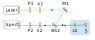
\includegraphics{../figures/setup_simplified.pdf}
	\caption{Used setup for photoluminescence measurements. 
	Changed from the reflection setup by adding the polarizers P$_{1,2}$ and retarders $\lambda_{1,2}$ to control the polarisation of the excitation and the detection.}
	\label{fig:pl setup}
\end{figure}
A setup to measure polarization-sensitive photoluminescence is illustrated in \autoref{fig:pl setup}.
The excitation laser at \SI{532}{nm} or \SI{647}{nm} is polarization-controlled using the polarizer P$_1$ and the retarder $\lambda_1$.
The mirror M$_1$ with the beam splitter BS$_2$ are aligned to minimize the reflection angle, to preserve the polarization as much as possible.
The beam splitter BS$_2$ is a polka dot mirror because it minimizes the changes in polarization compared to a glass wedge.
The detection path to the spectrometer is also polarization controlled with the retarder $\lambda_2$ and the polarizer P$_2$.\\
The retarders were configured to excite with circular polarization and detect with linear polarization or vice versa to prevent any bias in the excitation.
While this may not be necessary given that the excitation polarization is lost in the complex luminescence process \cite{NiPS3_linear}, it is a good practice to ensure that the measurements are not biased.

\begin{figure}
	\centering
	\includegraphics{../figures/2023-12-10 Combined PL.pdf}
	\caption{Measured Photoluminescence spectra at \SI{10}{K}. The sharp main peak of NiPS$_3$ allows for the detection of small changes in the energy.}
	\label{fig:pl}
\end{figure}
\autoref{fig:pl} depicts the photoluminescence spectra of various samples at \SI{10}{K}.
A main photoluminescence peak is observed, with different widths for the different materials. 
This peak can be explained by the neutral exciton photoluminescence process in NiPS$_3$ and CrPS$_4$ \cite{NiPS3_exciton,CrPS4_pl}, as it is below the bandgap.
Next to the main peak, multiple smaller peaks are visible.
These are more complex structures such as excitons in higher energy levels, charged excitons, or biexcitons \cite{CrPS4_pl, NiPS3_exciton,NiPS3_anisotropic, NiPS3_coherent}.
For this project, only the respective main peak is considered.\\
Despite exfoliation to remove the rough surface, no photoluminescence was detected for FePS$_3$ which is not consistent with the findings reported in \cite{FePS3_pl}.

\begin{figure}
	\centering
	\begin{subfigure}{2.5in}
		\includegraphics{../figures/2024-04-06 NiPS3 excitation power dependence.pdf}
		\caption{NiPS$_3$}
	\end{subfigure}
	\begin{subfigure}{2.5in}
		\includegraphics{../figures/2023-12-14 CrPS4 excitation power dependence.pdf}
		\caption{CrPS$_4$}
	\end{subfigure}
	\caption{Changes of the photoluminescence spectrum for different excitation power at \SI{10}{K}.}
	\label{fig:pl power dependence spectra}
\end{figure}
It is standard practice to use an excitation power in the range of \SI{5}{uW} to \SI{5}{mW} to prevent damage to the sample \cite{NiPS3_anisotropic, NiPS3_exciton}.
However, the damage threshold is dependent on the power density, and neither the beam size nor the damage threshold is known.
In order to get an understanding of the saturation of the sample the power scaling was measured.
The resulting spectra for different excitation powers are shown in \autoref{fig:pl power dependence spectra}.
No unexpected drastic changes that would indicate damage to the sample are visible.

\begin{figure}
	\centering
	\includegraphics{../figures/2024-04-19 excitation power dependence of main pl line.pdf}
	\caption{Excitation power dependence of the integrated main photoluminescence peak at \SI{10}{K} with a quadratic and power law fit. }
	\label{fig:pl power dependence}
\end{figure}
To gain a more comprehensive understanding, the intensity of the main peak can be integrated and plotted relative to the excitation power in \autoref{fig:pl power dependence}.
For NiPS$_3$, a quadratic function fitting indicates a linear scaling that begins to saturate at higher excitation powers.
For CrPS$_4$, the scaling is faster than linear, which can be explained by a scaling probability of creating biexcitons additionally to the exciton photoluminescence process \cite{biexciton}. \\
Since a power law fit is commonly used to describe the scaling the fit is also shown.\\
In order to achieve a good signal-to-noise ratio while avoiding saturating the sample, the excitation power was selected to be in the range of \SI{1}{} to \SI{4}{mW}.
Even when illuminated with \SI{20}{mW}, the sample did not exhibit any signs of damage.\\
However, following multiple measurements, the photoluminescence ceased in some NiPS$_3$ flakes.
This is not due to the excitation, as this also occurred in flakes that were not excited.
It is caused by oxidation during storage and manipulation of the samples.
There were no visible changes to those samples on optical microscope images.

\section{Measurement Setup}
\begin{figure}
	\centering
	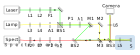
\includegraphics{../figures/setup.pdf}
	\caption{Detailed schematic of the entire measurement setup.}
	\label{fig:schematic full}
\end{figure}
The optical table had a few additional components not depicted on the simplified schematic \autoref{fig:pl setup}.
The full schematic is presented in \autoref{fig:schematic full}.

The sample $S$ could be illuminated with a fiber-coupled array of diode lasers to excite the photoluminescence or a fiber-coupled halogen lamp to enable imaging of the sample with a camera, and subsequently a stronger white LED for the same purpose.
The lenses $L_{1-4}$ were used to expand the cross-section of the illuminating beam in order to utilize the entire aperture of $L_5$.\\
$F_1$ was an interference film filter used to block out the detection wavelengths from the excitation light.
The aperture $A_1$ was mounted off-center to illuminate the sample in a dark-field configuration, thereby increasing the contrast in the camera image.
These two illumination paths were combined with cube beam splitters BS$_1$.
The polarizer P$_1$ and the retarder $\lambda_1$ were used to control the polarization of the light in the excitation path.
Then the mirror $M_1$ and the beam splitter BS$_2$ were used to introduce the light into the detection path in a way that minimized the alteration of the polarization, by minimizing the reflection angle.\\
To get more light for the camera, $M_1$ could be flipped out and $M_3$ could be flipped in.
This obstructs the spectrometer and compromises the polarization of the light, but increases the intensity by a factor of two.
$BS_3$ was just used to image the surface of the sample with the camera. 
It was a film beam splitter with a large aperture that had to be removed for polarization-sensitive measurements, as it is strongly polarizing.\\
The objective lens $L_5$ was mounted on an x-y-z piezo stage in the cryostat to move and focus on different flakes of the sample.\\
The cryostat and the magnet are combined in a single unit since the \SI{10}{T} superconducting magnet needs a helium reservoir.
The sample was in a variable temperature insert with a controllable helium cooling flow and an electric heater.\\
The light from the sample then goes through the retarder $\lambda_2$ and the polarizer P$_2$ to control the analyzed polarization.
The retarder $\lambda_2$ was mounted on a computer-controlled rotation stage.\\
The light then was focused by the lens $L_7$ into the spectrometer.
$L_7$ had a focal length of \SI{20}{cm} arbitrarily chosen by the previous user.
The interference filter $F_2$ was used to block out the excitation light from the spectrometer and is placed as close to the spectrometer as possible to block out all the stray excitation light.\\
The used spectrometer was a \SI{500}{nm} Czerny-Turner imaging spectrometer (ANDOR SR-500i) with a piezo-cooled CCD sensor and a 1200 lines/mm grating.


\chapter{Results}

\section{NiPS$_3$}
\begin{figure}
	\centering
	\includegraphics{../figures/2024-04-10 NiPS4 splitting.pdf}
	\caption{
		Photoluminescence intensity in NiPS$_3$ for different polarization directions $P$ to applied external magnetic field $H$ at \SI{5}{K}.\\
		For $P\parallel H$ the splitting $\Delta E$ is larger than for $P\perp H$.
	}
	\label{fig:NiPS3 splitting}
\end{figure}
First, NiPS$_3$ was investigated with polarization-resolved photoluminescence spectroscopy due to the sharp photoluminescence (PL) peak, which facilitates the detection of small changes in the energy.
This was done with exfoliated flakes on a Si/SiO$_2$ substrate for easier handling.

When an external magnetic field $H$ is applied to the sample in the natural $a$-$b$ plane of the crystal, the main photoluminescence line observed from the plane normal splits into two lines.
This is shown in \autoref{fig:NiPS3 splitting} for different detection polarizations $P$.\\
The amount of splitting $\Delta E$ is different for different polarization directions.
In the polarization direction where the external magnetic field $H$ is aligned with the electric field of the photoluminescence signal $P\parallel H$, the splitting $\Delta E$ is larger than in the perpendicular direction $P\perp H$.

\begin{figure}
	\centering
	\includegraphics{../figures/2024-04-21 NiPS3 DeltaE.pdf}
	\caption{$\Delta E$ measured with bi-gaussian fit. The splitting is largest for $P\parallel H$ and high magnetic field and decreases with increasing angle and lower field.}
	\label{fig:NiPS3 delta E}
\end{figure}
To directly determine $\Delta E$, the sum of two Gaussian peaks was fitted, with the peaks centered at $E\pm \nicefrac{\Delta E}{2}$ with the same amplitudes $I$ and widths $\sigma$.
Given that the linewidth is significantly narrower \cite{NiPS3_magnon_gap} than the resolution of the spectrometer, $\sigma$ was held constant over the field and polarization angle.
$E$ and $I$ were fitted independently for each measurement over field and polarization angle, as the turning retarder and the field-dependent moving sample holder altered the position of the focus on the spectrometer and the focus on the sample, thereby changing $E$ and $I$ respectively.
The resulting splitting $\Delta E$ is shown over the field and polarisation angle in \autoref{fig:NiPS3 delta E}.

\begin{figure}
	\centering
	\begin{subfigure}{4in}
		\includegraphics{../figures/2024-04-18 NiPS4 splitting 10K.pdf}
		\caption{10K: Many overlaid splitting curves caused by poly-crystalline flakes.}
		\label{fig:NiPS3 10K}
	\end{subfigure}
	\begin{subfigure}{4in}
		\includegraphics{../figures/2024-04-18 NiPS4 splitting 10K multiple flakes.pdf}
		\caption{10K: Two overlapping splitting curves for 2 crystal flake.}
		\label{fig:NiPS3 10K multiple flakes}
	\end{subfigure}
	\begin{subfigure}{4in}
		\includegraphics{../figures/2024-04-18 NiPS4 splitting 50K.pdf}
		\caption{50K: The line is too broad to observe the splitting.}
		\label{fig:NiPS3 50K}
	\end{subfigure}
	\caption{Splitting of the NiPS$_3$ photoluminescence line at different temperatures and different flakes.}
	\label{fig:NiPS3 multiple temperatures}
\end{figure}
This measurement was repeated for different samples and at different temperatures.
Representative results are shown in \autoref{fig:NiPS3 multiple temperatures}.
In most flakes, the splitting was not as clear as in \autoref{fig:NiPS3 splitting}.
It was either a broadening of the line as shown in \autoref{fig:NiPS3 10K} or multiple overlapping splitting curves as shown in \autoref{fig:NiPS3 10K multiple flakes} for \SI{50}{K}.\\
At higher temperatures, the photoluminescence peak was broader and the splitting was not visible, as shown in \autoref{fig:NiPS3 50K}.
Above \SI{50}{K} the photoluminescence could not be measured over the field, and thus the phase transition to paramagnetic at the Néel temperature of \SI{155}{K} \cite{MPS_magnetism} can not be observed with this method.\\
No hysteresis was observed over the magnetic field in any of the measurements.

\clearpage

\begin{figure}
	\centering
	\begin{subfigure}{\textwidth}
		\centering
		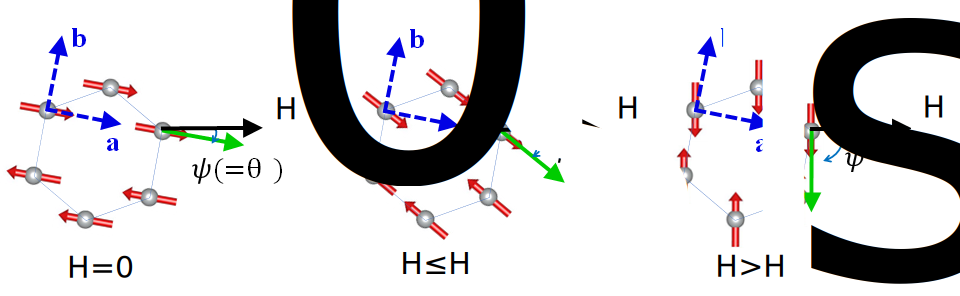
\includegraphics[width=.8\textwidth]{../figures/NiPS3_magnon_S2.png}
		\caption{Model for the photoluminescence signal in NiPS$_3$, with the spins of the Ni$^{2+}$-ions in the $a$-$b$ crystal plane. Adapted from \cite[Figure S2]{NiPS3_magnon_gap}.}
		\label{fig:NiPS3 linear model}
	\end{subfigure}
	\begin{subfigure}[t]{2.5in}
		\centering
		\includegraphics{../figures/2024-04-21 NiPS3 single polarisation.pdf}
		\caption{Recorded data for $P\parallel H$ at \SI{5}{K}, with fit for $\Delta E$ with $\theta_0 = \SI{27}{\degree}$ according to model \autoref{eq:NiPS3 model} from \cite{NiPS3_magnon_gap}.
		The model fits the data well if only one polarization is selected.
		}
		\label{fig:NiPS3 model}
	\end{subfigure}
	\begin{subfigure}[t]{3in}
		\centering
		\includegraphics{../figures/2024-04-07 NiPS3 polarisation.pdf}
		\caption{
			Integrated photoluminescence signal of the main peak for different polarizations. 
			With a $\cos^2$ fit, to show the polarization axis. 
			The $a$ and $b$ crystal axis are inferred from the polarisation at $H=0$ \cite{NiPS3_linear}.
			The polarisation rotates from perpendicular to the $a$ crystal axis to perpendicular to the magnetic field. 
		}
		\label{fig:NiPS3 polarisation peanut}
	\end{subfigure}
	\caption{Different models for the photoluminescence signal in NiPS$_3$.}
\end{figure}
To understand the observed splitting of the photoluminescence line, a model from \cite{NiPS3_magnon_gap} can be used, as the splitting was already observed there. 
A mean-field biaxial antiferromagnet model was proposed, that defines the angle $\psi$ shown in \autoref{fig:NiPS3 linear model} between the spin of the $Ni^{2+}$-ions and the external magnetic field $\vec{H}$.
For $H=0$ the spin aligns with the $a$-crystal axis, and thus, the initial angle $\theta_0=\psi\left(H=0\right)=\measuredangle(a, H)$ can be defined.
The coupling constants along the axis of the model result in an effective $g$ factor and a spin-flop field $H_\text{sf}$.
Consequently, the proposed model \autocite{NiPS3_magnon_gap} yields the following expressions for the angle $\psi$ and the splitting $\Delta E$:
\begin{align}
	\tan 2\psi &= \frac{\sin 2\theta_0}{\cos 2\theta_0 - \frac{H}{H_\text{sf}}^2}\\
	\Delta E &= \mu_B g H \cos \psi
	\label{eq:NiPS3 model}
\end{align}
This model does not describe polarization-resolved differences as $\Delta E$ is independent of the polarization angle.
This is not consistent with the experimental observations, where the splitting is dependent on the polarization angle.\\
Nevertheless, by taking into account only one polarization, the model describes the data shown in \autoref{fig:NiPS3 model}.
Even the same $H_\text{sf} = \SI{10.55}{T}$ and $g=\SI{2.0}{}$ from \autocite{NiPS3_magnon_gap} are found to correctly fit the data.\\
Within this model, the overlaid splitting curves in \autoref{fig:NiPS3 10K multiple flakes} can be understood as poly-crystalline or cracked flakes with rotated orientations of the $a$ and $b$ crystal axis and therefore different splitting curves.
This was confirmed by manufacturing a sample with more exfoliation steps to get thinner flakes, which yielded clearer splitting curves.

The non-zero linear polarisation degree of the observed photoluminescence is related to the nature of the underlying optical transition.
The main photoluminescence peak is caused by the transition from the Zhang-Rice triplet to the Zhang-Rice singlet state \cite{NiPS3_coherent}.
The spin orientations of the free electrons in the Ni $d$ orbital and the S $p$ orbital is the same for the triplet state and the opposite for the singlet state \cite{NiPS3_coherent}, which results in a change in angular momentum during the transition.
The difference in angular momentum $\Delta S$ is parallel to the spin alignment axis in the $a$-$b$ plane.
$\Delta S$ is carried away by a circularly polarized photon emitted in the $a$-$b$ plane and is not detected \cite{NiPS3_linear} in the perpendicular direction.
Viewed from the plane normal, the transition is a changing dipole that emits a linearly polarized photon with a polarization perpendicular to the spin alignment \cite{NiPS3_linear}.\\
In previous studies \cite{NiPS3_linear}, the linear polarization of the photoluminescence showed a magnetic-field-dependent rotation of the polarization from perpendicular to the $a$ crystal axis to perpendicular to the magnetic field.
This is reproduced in \autoref{fig:NiPS3 polarisation peanut}, which depicts the main peak of the photoluminescence signal measured with different polarisation angles and a $cos^2$ fit. The peak intensity was integrated from \SIrange{1.4732}{1.4768}{eV}. 

\begin{figure}
	\centering
	\includegraphics{../figures/2024-04-09 NiPS3 polarisation Splitting.pdf}
	\caption{Results from the $\cos^2$ fit for the photoluminescence spectra of NiPS$_3$ at \SI{5}{K}. The polarization of the photoluminescence peak does not behave uniformly.}
	\label{fig:NiPS3 polarisation splitting}
\end{figure}
However, the peak does not behave uniformly.
To examine the polarization direction, the data can be displayed by fitting the $\cos^2$ function for every wavelength and field individually.
The average intensity, polarization angle, and degree can then be extracted.
This is shown in \autoref{fig:NiPS3 polarisation splitting}.\\
As previously stated the photoluminescence line splits less when $P\perp H$ than when $P\parallel H$.
In the $\measuredangle P, H$-panel this is evident as a rotation of the polarization in the center of the line from $30$ to \SI{90}{\degree}.
The photoluminescence background below the main peak is polarized parallel to the magnetic field, resulting in an angle of $0$ or \SI{180}{\degree}.
In between there is a visible line where the angle is \SI{45}{degree}.
This simplifies the presentation of the data, as two images in \autoref{fig:NiPS3 splitting} are combined into one.\\
In order to quantify the degree of polarization, it is necessary to define a reference level.
The background level was selected as the photoluminescence signal next to the peak, evaluated as the mean between \SIrange{1.442}{1.467}{eV}.\\
The much lower polarization degree in \autoref{fig:NiPS3 polarisation splitting} compared to near unity in \cite{NiPS3_anisotropic} can be again explained by the polycrystalline nature of the flakes with rotated orientations of the crystal axis within the flakes and therefore different polarization directions.

Altogether, the linear polarization-resolved photoluminescence measurement shows that the luminescence process is more complex than previously understood \cite{NiPS3_coherent,NiPS3_magnon_gap} and more theoretical work is needed to explain it fully.

\section{CrPS$_4$}
\begin{figure}
	\centering
	\includegraphics{../figures/2024-04-09 CrPS4 linear Polarisation.pdf}
	\caption{Linear polarization of CrPS$_4$ photoluminescence spectrum at \SI{10}{K} over external magnetic field in plane. No change in the spectrum or the linear polarization is observed.}
	\label{fig:CrPS4 linear}
\end{figure}
Following studies of NiPS$_3$, CrPS$_4$ was examined next, as the photoluminescence behavior of the material under a magnetic field was not yet documented.
The photoluminescence signal in CrPS$_4$ exhibited a notably stronger and broader profile compared to NiPS3.
No observable splitting or displacement of the peak in the photoluminescence signal was detected in response to changes in the magnetic field. 
Additionally, even though the photoluminescence signal in CrPS$_4$ was strongly linear polarization (see \autoref{fig:CrPS4 linear}), no rotation over the external magnetic field was observed.


\begin{figure}
	\begin{subfigure}[t]{3.5in}
		\vskip 0pt
		\includegraphics{../figures/2023-12-14 CrPS4 circular dichroism.pdf}
		\caption{Circular dichroism of the photoluminescence in CrPS$_4$.}
		\label{fig:CrPS4 CD}
	\end{subfigure}
	\begin{subfigure}[t]{2.5in}
		\vskip 0pt
		\includegraphics{CrPS4_magneto_tourque.pdf}
		\caption{Magnetisation measured using magneto torque. Adapted from \cite[Figure 2]{CrPS4_magnetic}.}
		\label{fig:CrPS4 magnetic}
	\end{subfigure}
	\caption{Comparison of circular dichroism of the photoluminescence line and the magnetization in CrPS$_4$. The circular dichroism is proportional to the magnetization.}
\end{figure}
The circular dichroism of the photoluminescence in CrPS$_4$ in \autoref{fig:CrPS4 CD},
had a clear non-hysterical change over the magnetic field.\\
It is evaluated by integrating the intensity over the main photoluminescence peaks from \SIrange{1.28}{1.39}{eV}.
This reduces noise and is necessary to measure such small differences with the spectrometer.
However, there is no significant difference in the circular dichroism over the wavelength, so the spectrometer is not essential for this measurement.
The selection of the background level for calculating the dichroism is straightforward, as there is no significant difference if it is taken sufficiently far away from the photoluminescence peak or without the excitation.

However, the measured circular dichroism signal correlates perfectly with magneto torque measurements of the magnetization (see \autoref{fig:CrPS4 magnetic} from \cite{CrPS4_magnetic}) in all measured magnetic field configurations and temperatures.
However, the corresponding authors have thus far not provided their data for quantitative comparison.
But at least from qualitative comparison, the circular dichroism of the photoluminescence line is proportional to the magnetization in CrPS$_4$.\\
Additional theoretical work is necessary to explain this effect.
The main photoluminescence peak is attributed to a simple transition between doublet states in the Cr$^{3+}$-ions in \cite{CrPS4_pl} and therefore the origin of the circular dichroism of the resulting emission is not clear.\\
Nevertheless, the observed phenomenon can already be used to optically measure the change in magnetization of the CrPS$_4$ subject to an external magnetic field.
The magnetic phase transitions are visible as distinct changes in the magnetization curve in \autoref{fig:CrPS4 CD}.
The spin-flop transition at \SI{.8}{T} and the spin-flip phase transition at \SI{7.5}{T} can be observed, matching the magneto torque measurements \cite{CrPS4_magnetic}.\\
The method is not yet suitable for absolute magnetization measurement, as the circular dichroism to magnetization ratio differs between flakes.
This might depend on the thickness of the flakes.


\begin{figure}
	\centering
	\includegraphics{../figures/2024-04-22 CrPS4 temperature series.pdf}
	\caption{Photoluminescence of CrPS$_4$ for different temperatures. The photoluminescence signal gets broader but is still visible up to room temperature.}
	\label{fig:CrPS4 temperature}
\end{figure}
At higher temperatures, the photoluminescence signal broadens and the intensity decreases, as shown in \autoref{fig:CrPS4 temperature}.
Differently to NiPS$_3$ the photoluminescence signal is visible up to room temperature.
This is promising for studying the phase transitions to paramagnetic at the Néel temperature of \SI{38}{K} \cite{CrPS4_magnetic},
which allows for this method to be used to study the entire magnetic phase diagram of CrPS$_4$.

In conclusion, the circular dichroism of the photoluminescence signal in CrPS$_4$ allows for fast and localized measurements of the magnetization, that were not possible with previous methods.


\clearpage
\subsection{Aligning Flakes}
\label{sec:aligning flakes}
\begin{figure}
	\begin{subfigure}{2.5in}
		\includegraphics{../figures/2024-01-23 rotating pl.pdf}
		\caption{First successful measurement.}
		\label{fig:alignment first}
	\end{subfigure}
	\begin{subfigure}{3.5in}
		\includegraphics{../figures/2024-01-29 rotating pl.pdf}
		\caption{Partially reproduced measurement on different substrates.}
		\label{fig:alignment second}
	\end{subfigure}
	\caption{Rotation of the linear polarization of the photoluminescence signal in CrPS$_4$ during cooling. The photoluminescence signal aligns in the same direction on some observed flakes.}
	\label{fig:alignment}
\end{figure}
After several days of measurements on the first CrPS$_4$ sample, the linear polarization of the photoluminescence signal from all the studied flakes was aligned in the same direction.
This is unexpected for out-of-plane magnetic field measurements, as there was assumed to be no inherent axis in the sample plane and therefore symmetry for the in-plane rotational degree of freedom.\\
This was measured more systematically by creating new samples without any alignment in the exfoliation process.
For this, the adhesive tapes were rotated to arbitrary angles at each subdivision step and the transfer step was performed multiple times at different angles.\\
Then the linear polarization of several flakes was recorded during the cooling process, with particular care taken to ensure that no bias for one axis was introduced in the measurement.
Images were taken at each temperature in order to determine if the entire flake rotated or just the photoluminescence signal. \\
The initial measurement presented in \autoref{fig:alignment first} confirmed that the photoluminescence of all recorded flakes, which were randomly oriented at room temperature, aligned close to a single orientation at temperatures around \SI{200}{K}.
No rotation was observed in the images of the flakes, indicating that just the photoluminescence signal was rotating.

It was suspected that the Si lattice of the Si/SiO$_2$ substrate introduces an alignment direction.
Therefore, a glass substrate was used, which should not have a preferred axis.  
The results are presented in \autoref{fig:alignment second}, along with a new Si/SiO$_2$ sample to reproduce the aforementioned result.
However, in this experiment not all flakes aligned, which indicates a significant variance in the sample preparation.
Nevertheless, the alignment directions are different, indicating that the directionality is not originating from the experimental setup.
The images of the flakes show no correlation between the alignment and the shape or size of the flakes. 
Furthermore, the alignment does not correlate with the distance to neighboring flakes or the substrate material.

\begin{figure}
	\centering
	\begin{subfigure}[t]{1.8in}
		\includegraphics{../figures/2024-04-19 AFM (a).pdf}
		\caption{Normal flake, with a smooth surface.}
		\label{fig:AFM normal}
	\end{subfigure}
	\begin{subfigure}[t]{1.8in}
		\includegraphics{../figures/2024-04-19 AFM (b).pdf}
		\caption{Thin, torn flake, with cracks in the surface.}
		\label{fig:AFM torn}
	\end{subfigure}
	\begin{subfigure}[t]{1.8in}
		\includegraphics{../figures/2024-04-19 AFM (c).pdf}
		\caption{Flake with a rough surface, possibly glue residue.}
		\label{fig:AFM rough}
	\end{subfigure}
	\caption{Atomic force microscopy images of CrPS$_4$ flakes.}
	\label{fig:AFM}
\end{figure}
Following the measurements, atomic force microscopy images of the samples were recorded.
The flakes had a thickness ranging from \SIrange{200}{700}{nm}, as shown in \autoref{fig:AFM}.

In the case of the sample where all flakes aligned, all flakes had a smooth surface like in \autoref{fig:AFM normal} and \autoref{fig:AFM torn}.\\
On the samples where not all flakes aligned, some flakes had a rough surface, as shown in \autoref{fig:AFM rough}.
This rough patch extended over the flakes' boundary to the bare substrate.
This is likely residue from the adhesive used in the exfoliation process.\\
Additionally, thinner flakes on the Si/SIO$_2$ substrate had cracks in the surface as shown in \autoref{fig:AFM torn}.
The observed cracks appear to be mechanical stress fractures.
The origin of these cracks, whether due to unequal thermal expansion or from the mechanical exfoliation process, remains unclear. 

The source of the alignment remains unknown. 
Further research is needed because the phenomenon can possibly have an unknown influence on similar measurements.

\chapter{Conclusion and Outlook}
In this work, several materials belonging to the family of transition metal phosphorus sulfides were studied.
First, the samples were prepared from bulk crystals by mechanical exfoliation.
This was followed by a thorough examination with several optical measurement techniques in order to identify the most promising method for studying the magnetic properties of these materials.
Polarization-resolved photoluminescence spectroscopy was identified as the most promising method.

The findings reveal a higher complexity in the photoluminescence process of the studied materials than was previously reported.\\
Specifically, the linearly polarized photoluminescence of NiPS$_3$ exhibits a distinct splitting for different polarization directions, challenging current models \cite{NiPS3_magnon_gap,NiPS3_linear,NiPS3_coherent}.
Consequently, the objective now is to find a model for the photoluminescence process that can account for these measurements.\\
The investigation into CrPS$_4$ uncovered a correlation between the circular dichroism of the photoluminescence signal and the magnetization.
The observed proportionality offers a novel method for measuring the magnetization that is faster and more localized than previous methods.
With this method phase transitions have been observed, indicating its potential for studying the entire magnetic phase diagram of CrPS$_4$.
However, this challenges our current understanding of the photoluminescence process in this material, necessitating further research into the underlying mechanisms.
As of the time of writing, additional data is being recorded by the group in Warsaw to enhance the reliability of the results.\\
During these measurements, an unexpected alignment of the linear polarization of the photoluminescence signal was observed in CrPS$_4$ during cooling.
Despite efforts, the cause of this alignment could not be identified within the scope of this work.
Understanding the mechanism behind this alignment is crucial, as it may have implications for similar experiments.
The proposed next steps in further investigation of this phenomenon include:
\begin{itemize}
	\setlength\itemsep{-0.5em}
	\item Capturing atomic force microscopy images post-exfoliation to determine whether flakes are already torn.
	\item Modifying the temperature during the transfer step in exfoliation to investigate potential correlations with the rough surface, thereby confirming the presence of glue residue.
	\item Washing away the glue to confirm its stabilizing effect on the flakes.
	\item Experimenting with substrates with diverse thermal expansion coefficients to assess potential influence on the alignment.
\end{itemize}
However, all these procedures necessitate a statistical argument, demanding numerous samples. 
Nonetheless, it presents an opportunity for a future student to continue.



\backmatter
\nocite{*}
\addcontentsline{toc}{section}{Bibliography}
\printbibliography

\section*{Data Availability}
All the recorded data and software used for the analysis and documentation are available publicly at \url{https://github.com/leoole100/bachelorarbeit_public}.


\clearpage
\thispagestyle{empty}
\section*{Eigenständigkeitserklärung}
Ich versichere hiermit, dass ich die anliegende Abschlussarbeit mit dem Thema:
\textit{Optical signatures of magnetic phase transitions in transition metal phosphorus sulfides}
selbständig verfasst und keine anderen Hilfsmittel und Quellen als die angegebenen benutzt habe.

Falls ich textgenerierende KI-Tools als Hilfsmittel verwendet habe, ist mir bewusst, dass ich allein für
die inhaltliche Richtigkeit von KI generierten Textpassagen und die Kennzeichnung von
Formulierungen und Ideen anderer Personen gemäß den Grundsätzen der guten wissenschaftlichen
Praxis verantwortlich bin. Die Stellen, die anderen von natürlichen Personen verfassten Werken (auch
aus dem Internet und oder anderen elektronischen Text- und Datensammlungen entnommen) dem
Wortlaut oder dem Sinn nach entnommen sind, habe ich in jedem einzelnen Fall durch Angabe der
Quelle bzw. der Sekundärliteratur als Entlehnung kenntlich gemacht.

Ich habe zur Kenntnis genommen, dass die Prüfungs- oder Studienleistung bei Täuschung über die
Eigenständigkeit oder durch Benutzung nicht zugelassener oder ggf. zugelassener aber nicht
ausreichend angegebener Hilfsmittel als „nicht bestanden (5,0)“ bewertet wird und dass in besonders
schwerwiegenden Täuschungsfällen der zuständige Prüfungsausschuss mich von der
Wiederholungsprüfung ausschließen kann mit der Folge des endgültigen Verlustes des
Prüfungsanspruchs.

Weiterhin versichere ich hiermit, dass die o.g. Arbeit noch nicht anderweitig als Abschlussarbeit einer
Diplom-, Bachelor- bzw. Masterprüfung eingereicht wurde. Mir ist ferner bekannt, dass ich bis zum
Abschluss des Prüfungsverfahrens die Materialien verfügbar zu halten habe, welche die
eigenständige Abfassung der Arbeit belegen können.

Die Arbeit wird nach Abschluss des Prüfungsverfahrens der Bibliothek der Universität Konstanz
übergeben und katalogisiert. Damit ist sie durch Einsicht und Ausleihe öffentlich zugänglich. Die
erfassten beschreibenden Daten wie z.B. Autor, Titel usw. stehen öffentlich zur Verfügung und können
durch Dritte (z.B. Suchmaschinenanbieter oder Datenbankbetreiber) weiterverwendet werden.

Als Urheber der anliegenden Arbeit stimme ich dem obigen Veröffentlichungsverfahren zu.

Konstanz, den 2. Mai 2024

\end{document}